\chapter{Ingebruikname}

\section{Uitpakken en aansluiten van de MEGA65}
\label{cha:setup}

Het is tijd om uw MEGA65-homecomputer in gebruik te nemen! De doos bevat het volgende:

\begin{itemize}
\setlength\itemsep{-0.75mm}
	\item MEGA65-computer	\item Voeding (zwart kastje met aansluiting voor de netspanning)	\item Dit boek, de MEGA65-gebruikershandleiding	\item Uw persoonlijke registratiecode, op een papiertje (mogelijk in de gebruikershandleiding opgeborgen)
\end{itemize}

Om uw MEGA65-computer te kunnen gebruiken, heeft u bovendien het volgende nodig:

\begin{itemize}
	\item Een televisie of computermonitor met een VGA- of digitale video-ingang, die een beeld van 480p (720x480) bij 60 Hz of 576p (720x576) bij 50 Hz kan weergeven	\item Een geschikte videokabel voor uw beeldscherm, ofwel VGA, ofwel digitale video
\end{itemize}

Wellicht wilt u ook de volgende zaken gebruiken om het meeste uit uw MEGA65 te halen:

\begin{itemize}
	\item Een beeldscherm met digitale video-aansluiting en ingebouwde audio, of actieve luidsprekers met een geschikte audiokabel met een 3.5 mm-audiojackstekker	\item Een microSD-kaart, type SDHC, met een grootte tussen 4GB en 32GB	\item Een RJ45-ethernetkabel en een netwerkrouter of -switch	\item Een joystick of gamepad die compatibel is met Commodore-computers, met een negenpins-connector (DE-9)\index{Joystick}	\item Een Commodore 1351-muis, een Amiga-muis of een moderne vervanging, zoals een \href{https://retrohax.net/shop/amiga/mouster/}{mouSTer}-USB-muisadapter\index{Commodore 1351-muis}\index{Commodore Amiga-muis}\index{mouSTer-adapter}
\end{itemize}

\newpage
\section{Aansluitingen aan de achterzijde}
\index{Behuizing!Aansluitingen}

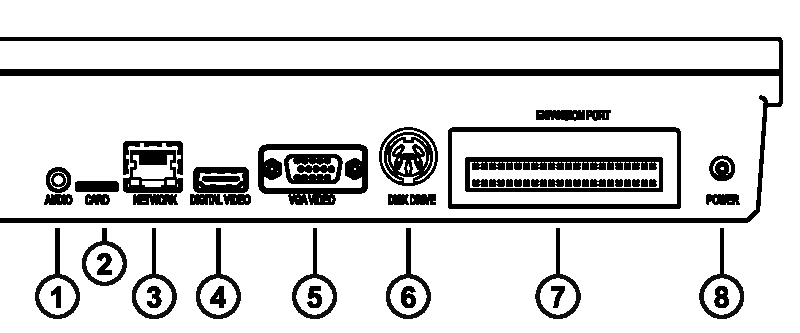
\includegraphics[width=\linewidth]{images/illustrations/mega65-rear.pdf}
\begin{center}
\setlength{\def\arraystretch{1.5}\tabcolsep}{6pt}
\begin{longtable}{ c | l}
	1	& 	3.5 mm-audiojack \\	2	& 	Externe microSD-kaartsleuf\\	3	& 	Netwerk-LAN-poort \\	4	& 	Digitale video-aansluiting (inclusief geluid) \\	5	& 	VGA-videoaansluiting \\	6	& 	Seriële IEC-bus-aansluiting voor schijfstations en printers \\	7	& 	Cartridge-uitbreidingspoort \\	8	& 	Voedingsaansluiting \\
\end{longtable}
\end{center}

\vspace{-1cm}

\section{Aansluitingen aan de zijkant}

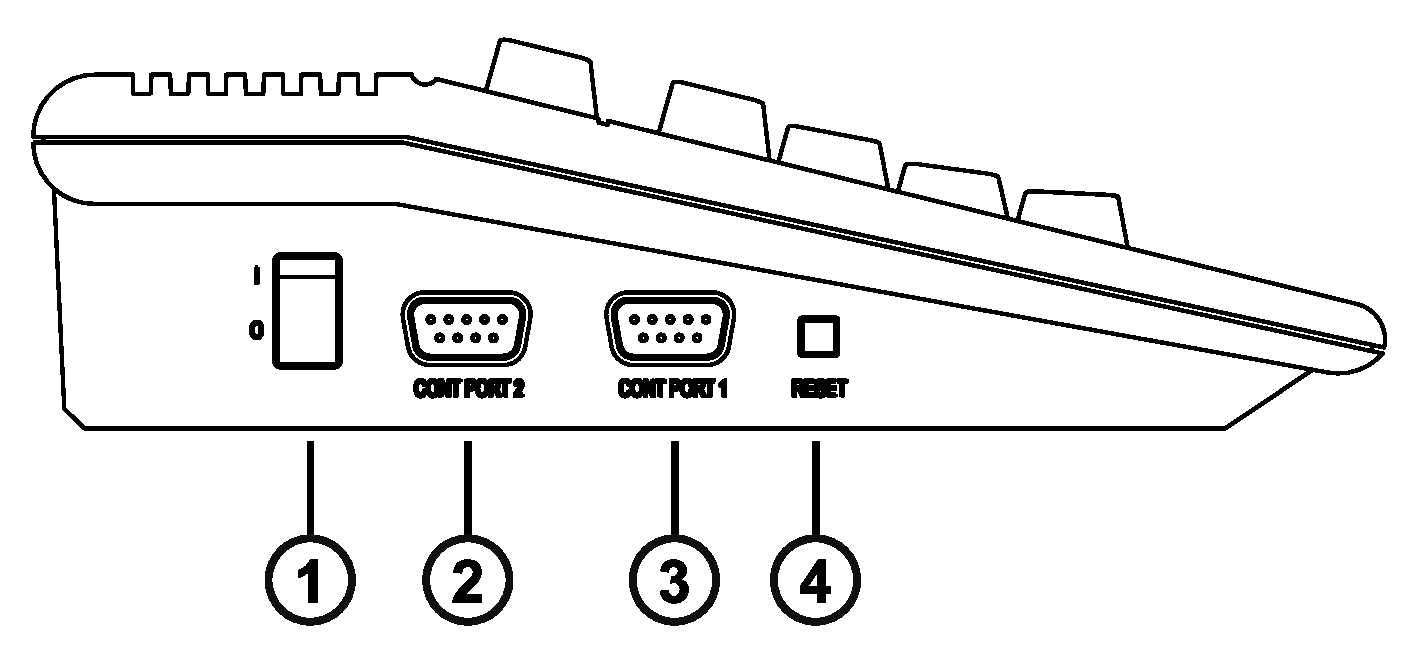
\includegraphics[width=\linewidth]{images/illustrations/mega65-side.pdf}

\begin{center}
\setlength{\def\arraystretch{1.5}\tabcolsep}{6pt}
\begin{longtable}{ c | l}
	1	& 	Aan/uit-schakelaar \\	2	& 	Controllerpoort 2 \\	3	& 	Controllerpoort 1 \\	4	& 	Resetknop \\
\end{longtable}
\end{center}

Op controllerpoorten 1 en 2 kunt u diverse randapparatuur aansluiten, zoals joysticks, peddels of muizen.

\newpage

\section{Beeldscherm en randapparatuur}

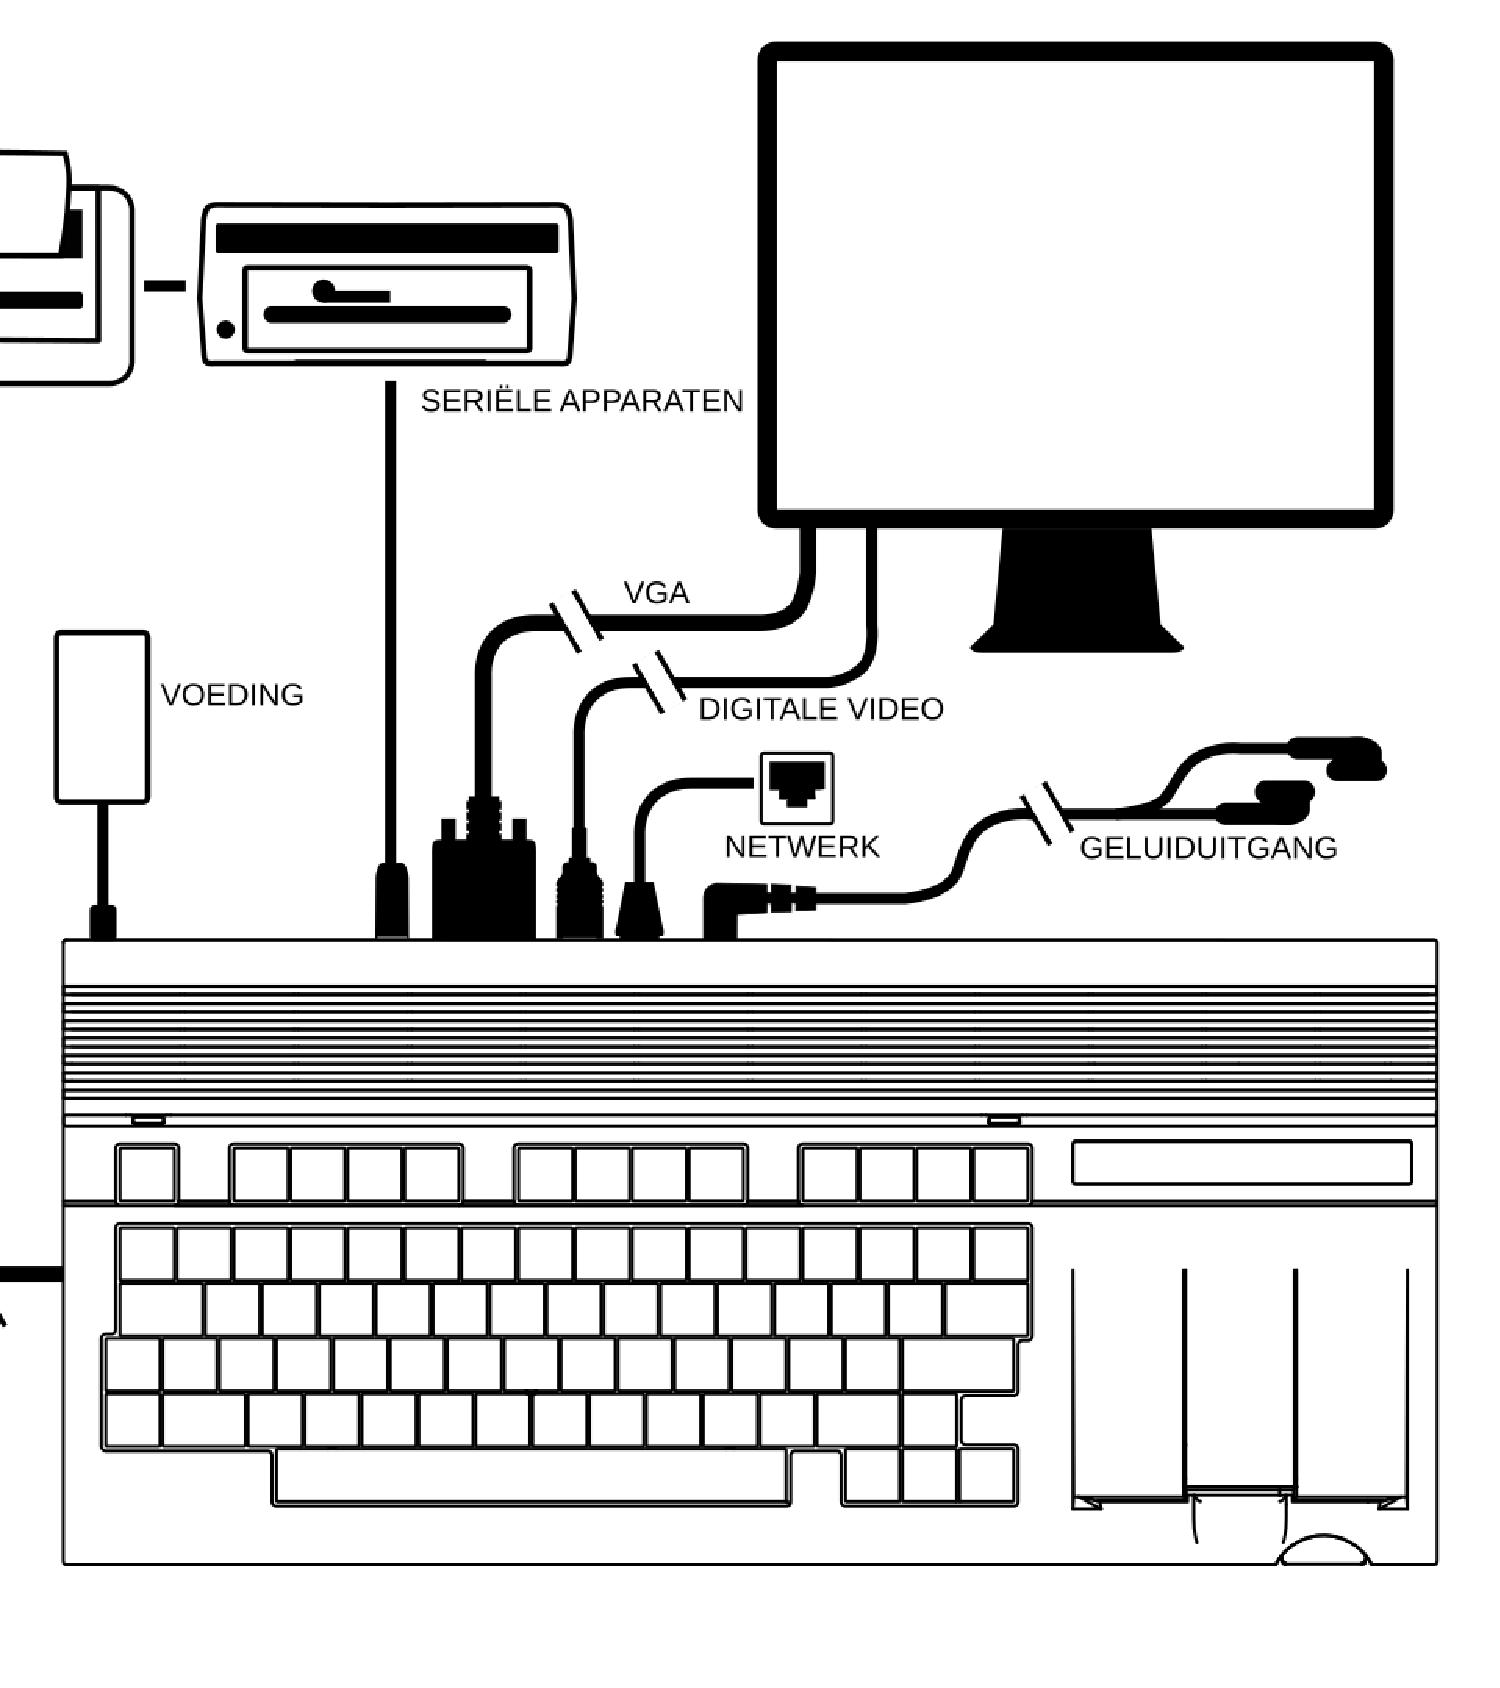
\includegraphics[width=\linewidth]{dutch/images/illustrations/mega65-top.pdf}

U sluit uw MEGA65 als volgt op een beeldscherm aan:
\index{Scherm!Aansluiten}

\begin{enumerate}
	\item Sluit de voeding aan op de voedingsaansluiting van de MEGA65.	\item Als u een VGA-monitor en een VGA-kabel hebt, sluit u het ene uiteinde aan op de VGA-poort van de MEGA65 en het andere uiteinde op uw VGA-monitor.	\item Als u een tv of monitor met een compatibele Digital Video-aansluiting hebt,\footnote{Het type Digital Video-aansluiting heeft een herkenbare commerciële naam van vier letters, doch het MEGA65-project heeft geen licentiekosten betaald om naar dit type met deze naam te verwijzen. Deze {\em Gebruikershandleiding} verwijst hiernaar als de ``Digital Video''-aansluiting.}\index{Digitale video} sluit u het ene uiteinde van uw kabel aan op de Digital Video-poort van de MEGA65 en het andere uiteinde op de Digital Video-poort van uw monitor. Als u een monitor met een DVI-aansluiting hebt, kunt u een Digital Video-naar-DVI-adapter gebruiken.
\end{enumerate}

\newpage
\section{Optionele aansluitingen}
\index{Schijfstations!Aansluiten}
\index{Aansluitingen!IEC}
\index{SD-kaarten!Locaties}
\begin{enumerate}
	\item De MEGA65 bevat een ingebouwd 3.5 inch-diskettestation. U kunt ook oudere Commodore{\textregistered}-diskettestations via de seriële IEC-bus aansluiten, zoals de Commodore 1541, 1571 of 1581. Sluit om deze stations te gebruiken het ene uiteinde van een IEC-kabel aan op het Commodore-diskettestation en het andere uiteinde op de schijfstationsaansluiting van de MEGA65. U kunt ook een SD2IEC-apparaat\index{SD2IEC-apparaat} of een Pi1541-apparaat aansluiten.\index{Pi1541-apparaat} Bij de meeste apparaten kunt u extra diskettestations of met Commodore compatibele printers aan elkaar koppelen.	\item U kunt uw MEGA65 met een standaard ethernetkabel aansluiten op een ethernetnetwerk.	\item Om naar audio van uw MEGA65 te luisteren, kunt u een 3.5 mm-audiojackkabel aansluiten op een audioversterker of een luidsprekersysteem. Als uw systeem over RCA-aansluitingen beschikt, hebt u een 3.5 mm-audiojack-naar-twin-RCA-adapterkabel nodig. De MEGA65 heeft tevens een ingebouwde versterker, zodat u een hoofdtelefoon kunt gebruiken.	\item U kunt een microSD-kaart, type SDHC tussen 4GB en 32GB, in de externe microSD-kaartsleuf aan de achterzijde van de MEGA65 steken. Zie voor meer informatie over het gebruik van de microSD-kaartsleuf ``Kennismaken met SD-kaarten'' op bladzijde \pageref{sec:introducing-sd-cards}.	\item Aan de onderzijde van de MEGA65 geeft een klein klepje toegang tot de interne SD-kaart en twee aansluitingen voor toekomstige hardware-uitbreidingen.
\end{enumerate}

\index{Real-time klok!Batterij plaatsen}
\subsection{De batterij van de real-time klok installeren}

De MEGA65 bevat een real-time klok, welke wordt gebruikt om de tijd en datum op het opstartscherm weer te geven, om tijdstempels toe te voegen aan bestanden die de MEGA65 op uw SD-kaarten schrijft en om de {\bf DT\$}\index{BASIC 65-variabelen!DT} en {\bf TI\$}\index{BASIC 65-variabelen!TI\$}-BASIC-variabelen voor gebruik in programma's te verschaffen. Deze klok gebruikt een CR2032-knoopcelbatterij om de tijd bij te houden wanneer de MEGA65 gedurende langere perioden van de voeding is losgekoppeld. De MEGA65 wordt niet met een batterij geleverd, om problemen met het internationaal verzenden van batterijen te vermijden.\footnote{Vroege modellen van de MEGA65 met de ``R3A''-printplaatrevisie (gemaakt in het jaar 2022) gebruiken een batterij van het type CR1220 voor de real-time klok en de batterij is vereist om de RTC te laten functioneren. Revisie ``R6'' (gemaakt in 2024) gebruikt een batterij van het type CR2032 en de batterij is optioneel voor normaal gebruik.}

{\bf De RTC-batterij is optioneel.} De MEGA65 kan de RTC zonder batterij draaiende houden, zelfs wanneer de computer gedurende meerdere dagen achter elkaar van de voeding is losgekoppeld. Met een batterij kan de computer de tijd gedurende veel langere perioden onthouden. U kunt de klok later altijd opnieuw instellen.

Schakel de computer uit om de batterij te installeren. Gebruik een kruiskopschroevendraaier om de behuizing te openen, waardoor het moederbord zichtbaar wordt.\index{Behuizing!Opening} De behuizing wordt bijeengehouden door drie schroeven, allemaal langs de onderkant van de voorzijde van de behuizing. Til, nadat de schroeven zijn verwijderd, voorzichtig de bovenste helft van de behuizing op. Let op de oriëntatie van de toetsenbordaansluiting en koppel deze vervolgens los.

De batterij bevindt zich tussen de controllerpoorten en de toetsenbordaansluiting.

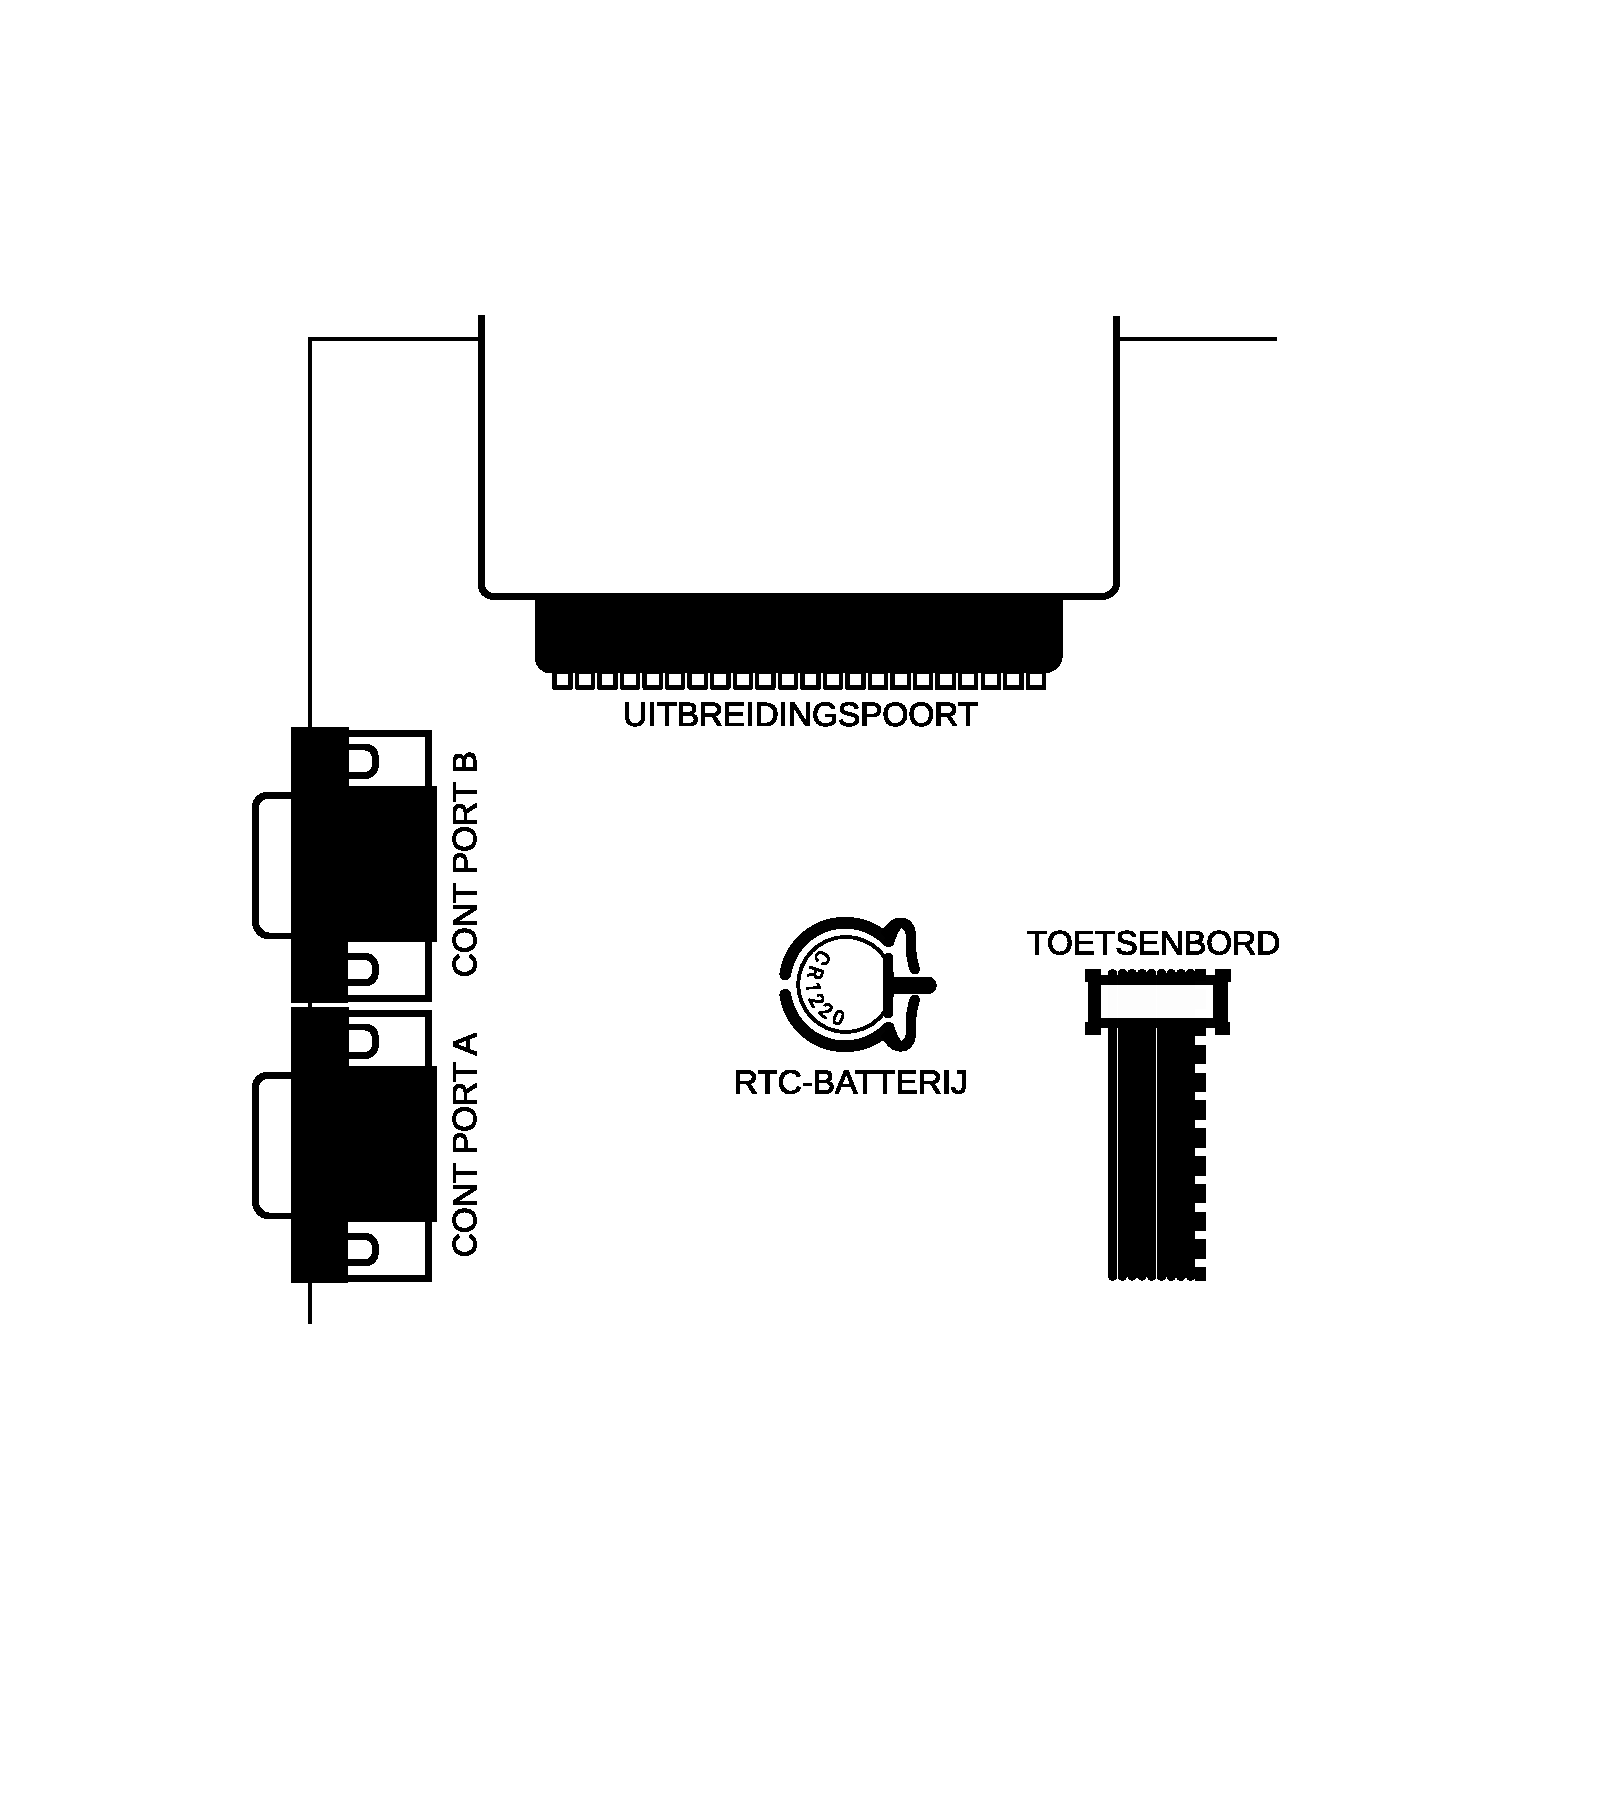
\includegraphics[width=\linewidth]{dutch/images/illustrations/rtc-battery-location.pdf}

Indien u een bestaande batterij verwijdert, duwt u de ontgrendelingshendel van de batterij aan de onderkant (de platte zijde) van de batterijhouder weg van de batterij om deze te verwijderen. Plaats de nieuwe batterij met de positieve zijde (gemarkeerd met {\bf +}) naar boven gericht en druk hem op zijn plaats.

Zodra u uw MEGA65 weer in elkaar hebt gezet, kunt u in het configuratiehulpprogramma de tijd instellen. Zie voor meer informatie over het instellen van de real-time klok het onderdeel over het configuratiehulpprogramma op bladzijde \pageref{sec:configuration-utility}.


\newpage

\section{De MEGA65 inschakelen}
\label{onboarding}

Schakel de MEGA65 in met de aan/uit-schakelaar aan de linkerkant van de computer.

Wanneer u uw MEGA65 voor het eerst inschakelt, toont de computer het scherm voor de initiële configuratie (``on-boarding'').\index{Configuratie!Introductie} Op dit scherm kunt u de tijd en de datum op de real-time klok instellen, de videomodus wijzigen en het geluid testen. Al deze instellingen kunt u later nog wijzigen.

\begin{center}
  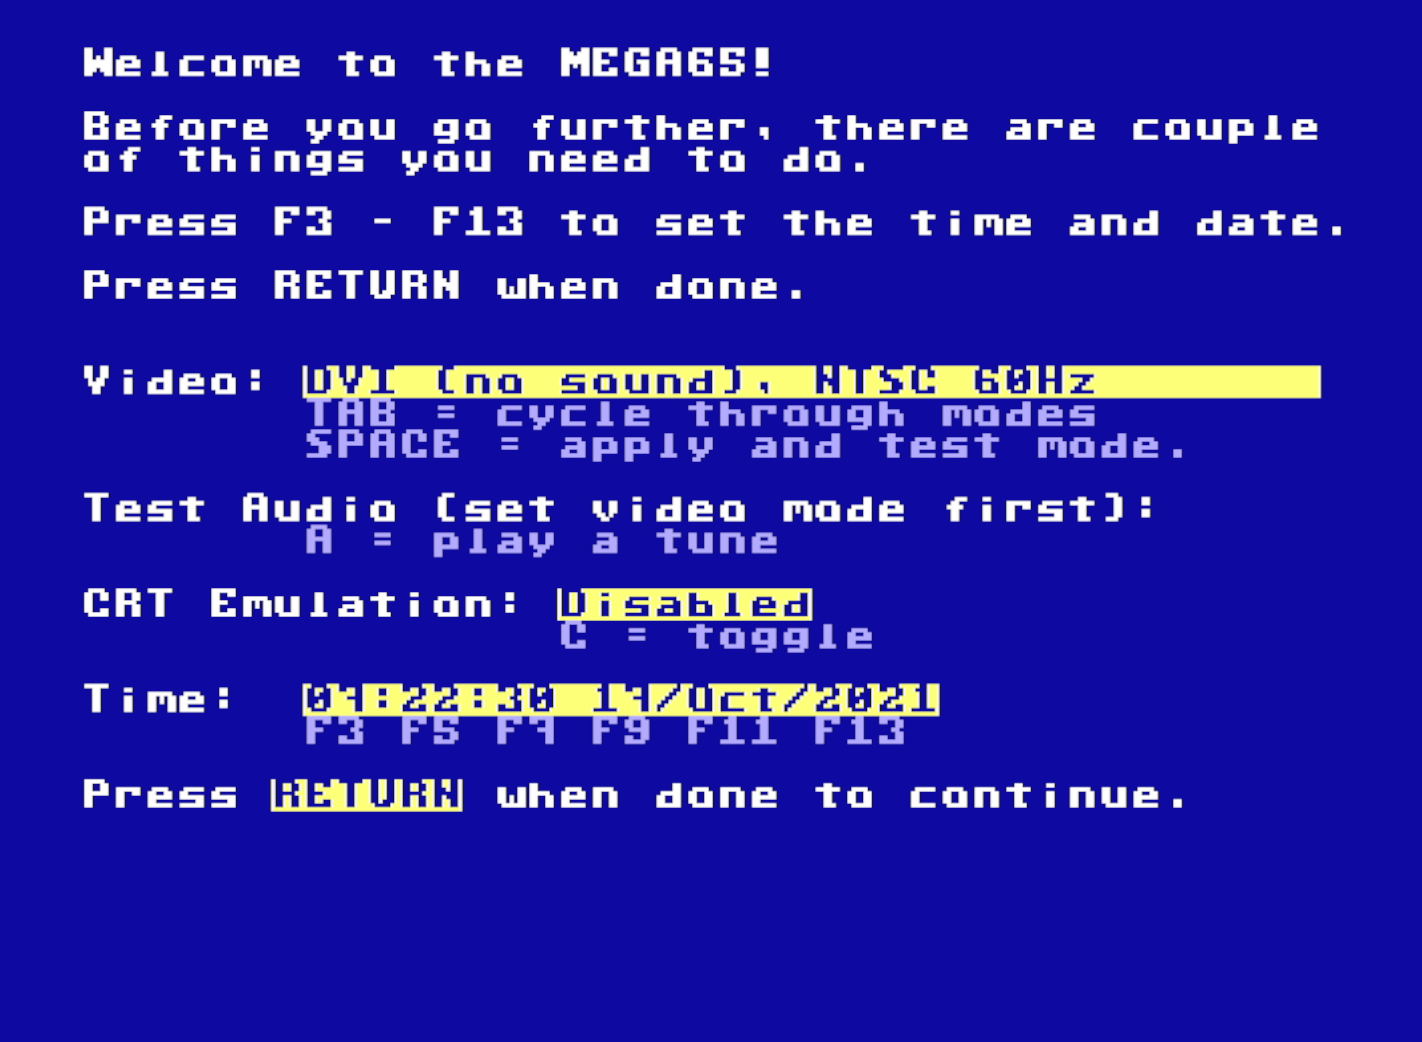
\includegraphics[width=0.7\linewidth]{images/img011_final_boot_01.png}
\end{center}

Voor videomodi kunt u kiezen tussen PAL-emulatie\index{PAL-schermmodus} en NTSC-emulatie\index{NTSC-schermmodus}. Daarnaast kunt u aangeven of uw Digital Video-beeldscherm geluid ondersteunt. Indien u de VGA-videouitgang gebruikt, heeft de Digital Video-geluidsmodus geen effect.

\underline{OPMERKING}: Een DVI-beeldscherm dat geen geluid ondersteunt, werkt niet met de ``enhanced''-geluidsmodus. Bij een dergelijk beeldscherm moet u een videomodus met ``no sound'' selecteren en een luidspreker op de 3.5 mm-audioaansluiting aansluiten.

PAL en NTSC zijn analoge videosignaalformaten die de resolutie en de verticale synchronisatiesnelheid van de videouitgang beïnvloeden, ook wanneer u een modern digitaal beeldscherm gebruikt. Uw beeldscherm ondersteunt mogelijk beide modi of slechts één van beide. U kunt dit scherm gebruiken om de modi met uw beeldscherm te testen.

Selecteer en test uw videoconfiguratie. Druk bijvoorbeeld op \specialkey{TAB} om naar de modus {\bf PAL 50Hz} over te schakelen.
\index{Scherm!PAL/NTSC instellen}
\begin{center}
  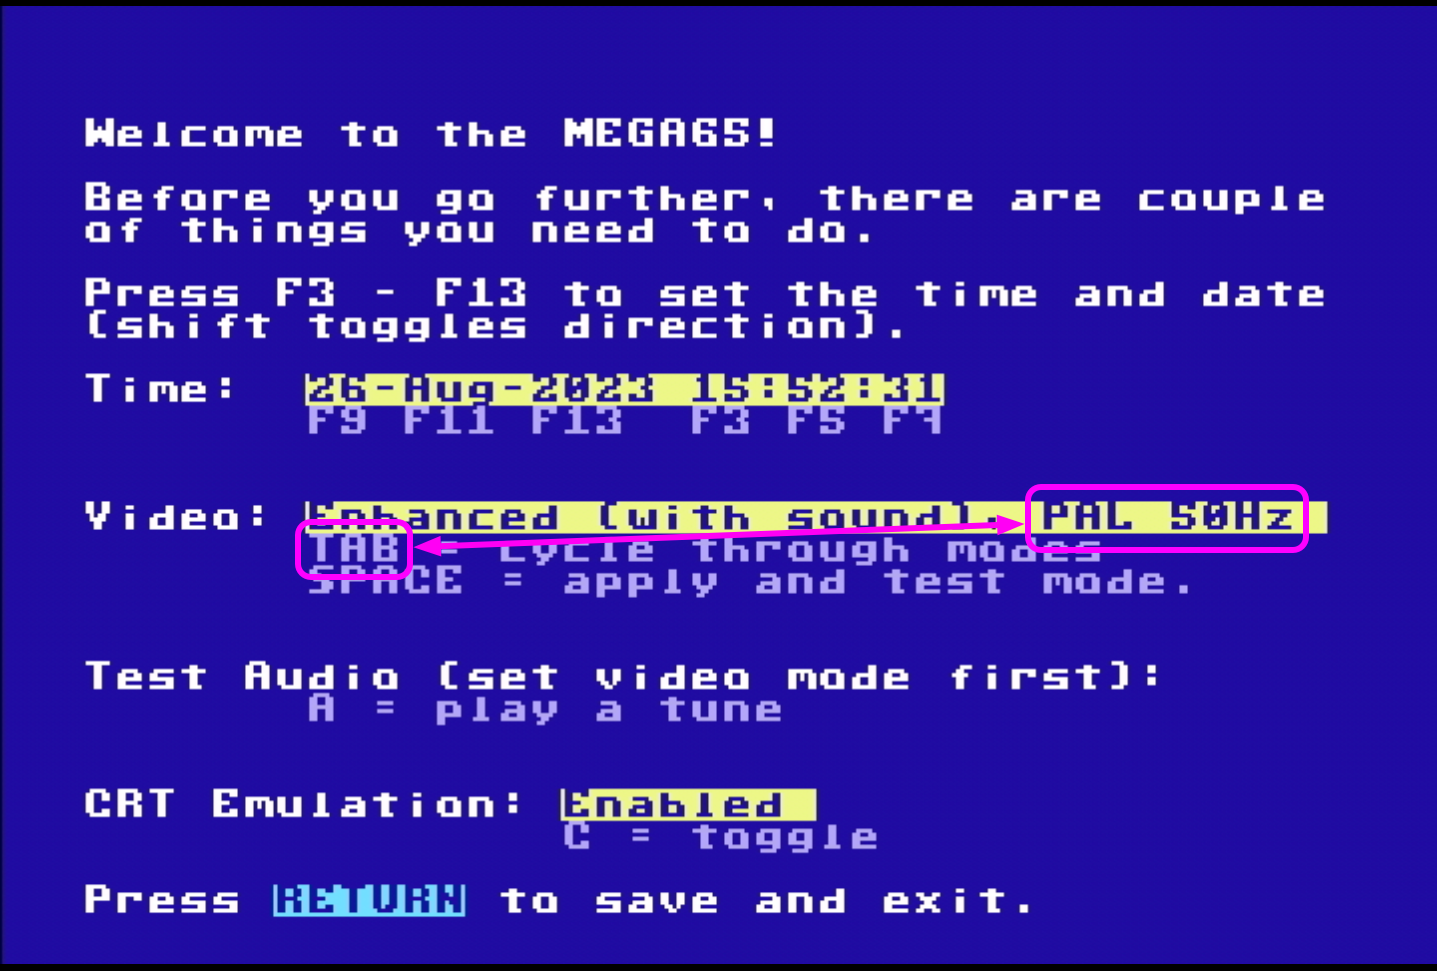
\includegraphics[width=0.7\linewidth]{images/img011_final_boot_02.png}
\end{center}

Druk op \megakey{SPACE} en vervolgens op \megakey{Y} om de nieuwe videomodus te testen.

\begin{center}
  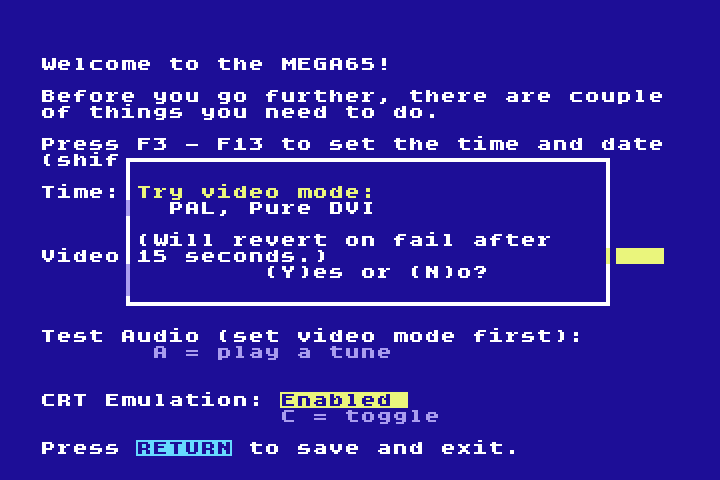
\includegraphics[width=0.7\linewidth]{images/img011_final_boot_03.png}
\end{center}

Druk op \megakey{K} om de nieuwe videomodus te behouden.

\begin{center}
  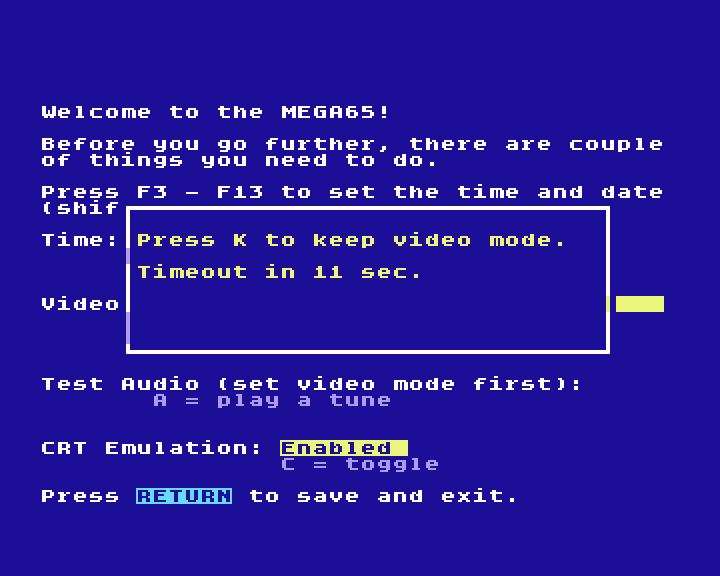
\includegraphics[width=0.7\linewidth]{images/img011_final_boot_04.png}
\end{center}

Maak van deze gelegenheid gebruik om uw geluidsopstelling te testen. Druk op \megakey{A} om een geluid af te spelen.

De optie ``CRT Emulation'' is een leuke keuze bij gebruik van een modern plat scherm. Deze optie voegt verticale tussenruimten toe tussen de pixels om de rasterlijnen van een beeldbuis na te bootsen. Probeer het om te zien of het u bevalt: druk op de toets \megakey{C} om de optie in en uit te schakelen.

Druk ten slotte op \specialkey{RETURN} om de configuratie af te ronden.

Zie voor meer informatie over het configureren van uw MEGA65 hoofdstuk \vref{cha:configuringyourmega}.

\section{De Intro Disk}
\index{Intro Disk}

Nadat u de initiële configuratie hebt afgerond, start uw MEGA65 het Intro Disk-menu. De Intro Disk is een verzameling software van de MEGA65-gemeenschap die enkele van de mogelijkheden van de computer demonstreert. Neem de tijd om door de menu's te bladeren en een aantal demo's uit te proberen. Druk na elke demo op de resetknop aan de linkerkant van de computer om terug te keren naar het Intro Disk-menu.

\begin{center}
  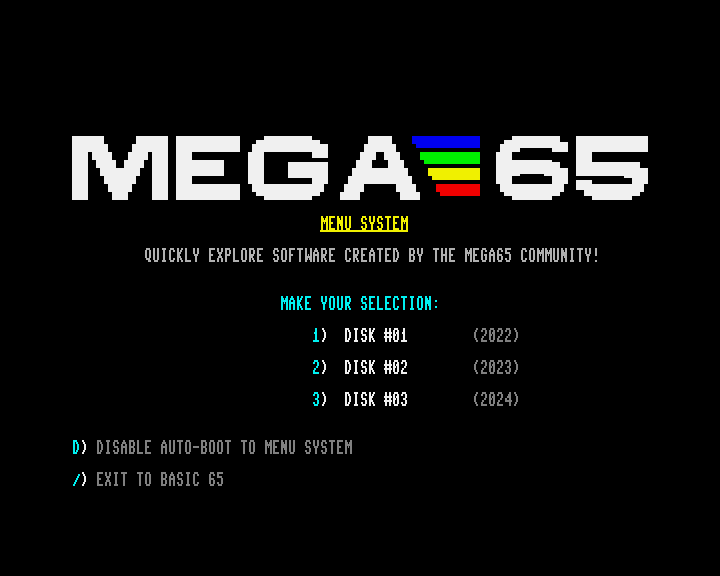
\includegraphics[width=0.7\linewidth]{images/demo_title.png}
\end{center}

Standaard opent het Intro Disk-menu telkens wanneer u de computer inschakelt. Zodra u meer vertrouwd bent met de MEGA65, wilt u dit wellicht uitschakelen. Druk bij het Intro Disk-menu op \megakey{D} om de automatische opstartfunctie van de Intro Disk uit te schakelen.\index{Intro Disk!Uitschakelen}

Druk op \megakey{/} (de schuine streep) om het Intro Disk-menu te verlaten en toegang te krijgen tot BASIC 65. Indien de automatische opstartfunctie van de Intro Disk is uitgeschakeld, gaat de MEGA65 bij het inschakelen rechtstreeks naar BASIC 65.

\begin{center}
  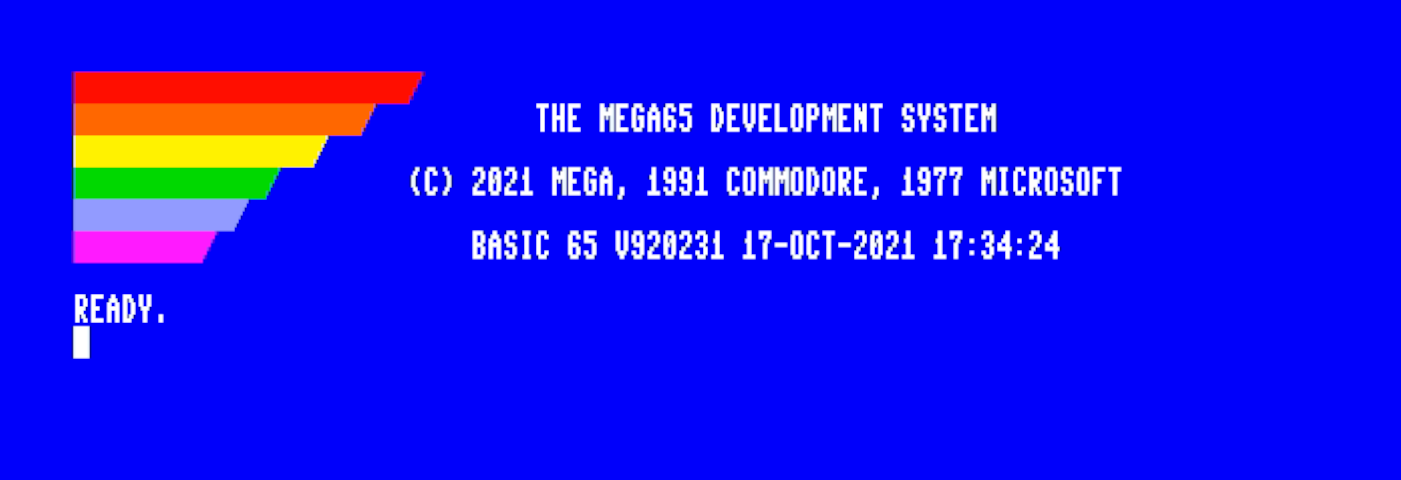
\includegraphics[width=0.7\linewidth]{images/img011_final_boot_06.png}
\end{center}

\section{De cursor}

Het knipperende blokje onder de \screentext{READY}-prompt\index{READY-prompt} wordt de \emph{cursor} genoemd. De cursor geeft aan dat de computer klaar is om invoer te ontvangen. Wanneer u toetsen op het toetsenbord indrukt, verschijnen de bijbehorende tekens op het scherm. De tekens verschijnen op de huidige cursorpositie en de cursor schuift na elke toetsaanslag een positie op.

Hier kunt u commando's typen waarmee u bijvoorbeeld een programma kunt laden. U kunt ook beginnen met het intypen van programmacode!
